\twocolumn

\begin{enumerate}
  	\setcounter{enumi}{2}
  	\item Решить неравенство
		\[log_{\frac{1}{4}} |\frac{x + 1}{x - 1}| > -1.\]
	\item Найти три первых члена бесконечно убывающей геометрической прогрессии, сумма которой 40 $\frac{1}{2}$, 
		а сумма первых четырех членов равна 40.
	 \item Около шара радиуса R описана правильная шестиугольная пирамида, боковая грань которой составляет
		 с плоскостью основания угол $\alpha$. Определить боковую поверхность и объем пирамиды.
\end{enumerate}

\begin{center}
	{\addfontfeatures{LetterSpace=30} Вариант 2}\\
	(все остальные специальности)
\end{center}

\begin{enumerate}
	\item Решить уравнение \[log_2^2 8x - log_2^2 4x + log_2^2 2x = log_2 64\]
	\item Решить уравнение \[ \cos(x+4\pi) + \sin(\frac{9\pi}{2} - 2x) - \sin(3x - \frac{\pi}{2}) = 0\]
	\item Решить неравенство \[\sqrt{2x + 15} < x.\]
	\item Сумма квадратов корней уравнения $4x^2 - ax + 1 = 0$ равна $\frac{17}{16}$, найти а.
	\item Боковые ребра правильной треугольной пирамиды составляют угол $\alpha$ с плоскостью основания и имеют длину l.
		Через одну из сторон основания проведено сечение, составляющее с плоскостью основания угол $\beta (\beta < \alpha)$ . 
		Вычислить площадь сечения.
\end{enumerate}

\begin{center}
	\textbf{Физика} \\
	{\addfontfeatures{LetterSpace=30} Билет 1}
\end{center}

\begin{enumerate}
	\item Равномерное движение по окружности. Линейная и угловая скорости. 
		Центростремительная сила и центростремительное ускорение.
	\item Понятие о волновой и квантовой природе света.
	\item Два точечных заряда $+q_1$ и $-q_2$  расположены в воздухе на расстоянии d друг от друга. 
		Найти напряженность и потенциал поля, создаваемого этими зарядами в точке А, находящейся на расстоянии $r_1$
		от положительного заряда и $r_2$ от отрицательного заряда. (Точка А не лежит на прямой, соединяющей заряды 
		$q_1$ и $q_2$.)
 \end{enumerate}

\begin{center}
	{\addfontfeatures{LetterSpace=30} Билет 2}
\end{center}

\begin{enumerate}
	\item Работа силы. Механическая энергия. Связь работы с изменением энергии. Единицы измерения энергии и работы.
	\item Цепная реакция. Выделение энергии при делении тяжелых ядер. 
	\begin{figure}[h]
		\centering
		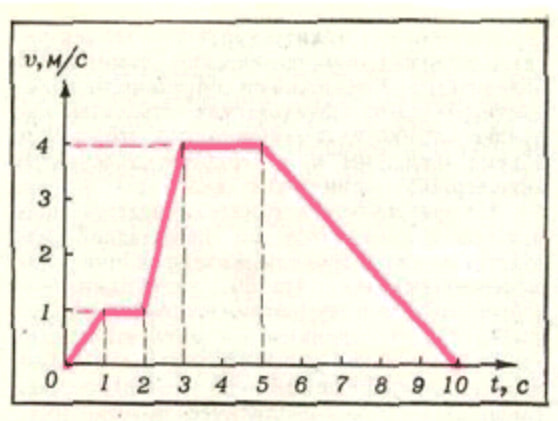
\includegraphics[width=1\linewidth]{pic_5}
		\caption{}
		\label{fig:circle}
	\end{figure}
	\item Движение точки задано графиком скорости (рис. 1). Определить среднюю скорость и среднее ускорение точки за 5 секунд. 
		По данному графику скорости точки построить график ускорения. 
\end{enumerate}

\begin{center}
	{\addfontfeatures{LetterSpace=30} Билет 3}
\end{center}

\begin{enumerate}
	\item Законы Бойля-Мариотта, Гей-Люссака, Шарля. Графики этих законов. Объединенный закон Бойля-Мариотта-Гей-Люссака.
	\item Магнитный поток. Электромагнитная индукция. Э. д. с. индукции. Закон Ленца. Устройство генератора переменного тока.
 \end{enumerate}

\textbf{\Large{\noindent Львовский \\ политехнический \\ институт}}

Львовский ордена Ленина политехнический институт - один из старейших высших технических учебных заведений страны, он был основан в 1844 году как техническая Академия, которая в 1877 году была переименована в Высшую политехническую школу, а в 1921 году- во Львовскую политехнику.

Бурное развитие вуза началось с сентября 1939 года, после воссоеденения западных областей Украины в едином Украинском Советском Социалистичеком государстве, когда Львовская политехника была реорганизована в политехнический институт. 

\newpage

\begin{tabular}{ |c| c| c| c|}
\hline
 &  $x_2<-1$ & $-1<x_2<1$ & $x_2>1$ \\
\hline
$x_1<-1$  &  $(+)(+)=+$  &  $(-)(+)=-$  &  $(-)(-)=+$ \\
$-1<x_1<1$  &  $-$  &  $(+)(+)=+$  &  $(+)(-)=-$ \\
$x_1>1$  &  $-$  &  $-$  &  $(+)(+)=+$ \\
\hline
\end{tabular}


